\documentclass[a4paper,11pt,oneside]{article}
\usepackage[ngerman]{babel} % für die deutsche Sprache
\usepackage[T1]{fontenc} % Schriftkodierung (Für Sonderzeichen u.a.)
\usepackage[utf8]{inputenc} % Für die direkte Eingabe von Umlauten im Editor u.a.
\usepackage{fancyhdr} % Für Kopf- und Fußzeilen
\usepackage{lmodern} % Schriftart "Latin Modern"
%\usepackage[normalem]{ulem} % Für das Unterstreichen von Text z.B. mit \uline{}
\usepackage[left=2cm,right=3cm,top=1cm,bottom=1cm,
textheight=245mm,textwidth=160mm,includeheadfoot,headsep=1cm,
footskip=1cm,headheight=14.599pt]{geometry} % Einrichtung der Seite 
\usepackage{setspace} % Paket zum Setzen des Zeilenabstandes
\usepackage{graphicx} % Zum Laden von Graphiken
\usepackage{amsmath}
\usepackage{amsthm}
\usepackage{amsfonts}
\usepackage{hyperref} % Hyperlinks im Inhaltsverzeichnis
\usepackage{pdfpages}
\usepackage{csquotes}
\usepackage{float}
\title{Titel}
\author{Tobias Magh}
\date{\today}

\usepackage[style=numeric,sorting=none]{biblatex} % Stil hier angeben
\addbibresource{Literatur.bib} % .bib Datei hier einbinden

\onehalfspacing

\begin{document}
	\pagestyle{fancy}
	\section*{Kurzanleitung zum erstellen und verwenden von PV-Look-up Tabellen in Plecs}
	Um ein beliebiges PV-Modul in Plecs zu simulieren muss zuvor ein Look-up Tabelle (LUT) generiert und in plecs eingebunden werden. Diese Kurzanleitung soll auf die dafür notwendigen Schritte eingehen.
	Für die Modellierung der Kennfelder wird das mathematische Model von U.Boeke \cite{Boeke} verwendet. Eine Look-up Tabelle wird mittels Skript generiert und in einem 3D-LUT-Block in Plecs geladen.
	\setcounter{section}{0}
	\section{Vorraussetzugen}
		Für die Modellierung werden zunächst folgende Daten über das PV-Modul benötigt:
		\begin{singlespace}
			\begin{itemize}
				\item Leerlaufspannung: $V_{OC}$
				\item Kurzschlussstrom: $I_{SC}$
				\item Spannung im Maximum Power Point(MPP): $V_{MPP}$
				\item Strom im MPP: $I_{MPP}$
				\item Leerlaufspannung bei geringer Sonneneinstrahlung (ca. 200W/m²): $V_{MIN}$
				\item Spannungstemperaturkoeffizient: $T_{CV}$
				\item Strom-Temperaturkoeffizient: $T_{CI}$
			\end{itemize} 
		\end{singlespace}
	
		\noindent
		Weiterhin werden die Programme Matlab\cite{MATLAB} oder GNU Octave benötigt. Alle begefügten Skripte wurden mit Octave Version 7.3.0 unter Linux getestet. Für die Verwendung mit Matlab müssen evtl. Änderungen vorgenommen werden.
	\section{Verwendung}
		\subsection{LUT generieren}
			In der Datei \enquote{pv\_lut.m} müssen zunächst die oben genannten Parameter des PV-Moduls eingegeben werden. Auch können hier z.B. Variablen für die Stützstellenanzahl der Kennlinien festgelegt werden. Für das Ausführen des Skripts sollten die Hinweise in den Kommentaren beachtet werden.\\ 
		\subsection{Ausgabe überprüfen}
			Die Binäre \enquote{pv\_lut.mat} Datei, welche im selben Ordner wie das Skript generiert wird, kann nun in Plecs eingebunden werden. Es ist allerdings ratsam das Ergebnis vorher zu überprüfen. Da es sich um eine Binärdatei handelt, kann diese nicht lesbar im Texteditor angezeigt werden. Mit dem beigefügten Skript \enquote{look\_into\_binary\_lut.m} können die Daten im Befehlsfenster von Octave angezeigt werden. Mit dem Skript \enquote{plot\_Isurf.m} wird das Kennlinienfeld als 3D-Plot für eine vom Nutzer eingegebene Temperatur angezeigt. Wichtig ist, dass das Skript im selben Ordner wie das LUT legt. Andernfalls müssen die Pfade im Code angepasst werden.
		
		\subsection{PV-Modul in Plecs}
			In Plecs wird das PV Modul durch ein 3D-Table Block und einer Idealen Stromquelle nachgebildet. Der Ausgang des 3D-Table wird dabei mit dem Eingang der \enquote{Current Source (controlles)} verbunden. Dieses System kann wiederum als ein PV-Block-Subsystem in einer Schaltung verwendet werden. Ein Beispiel dafür ist in der Datei \enquote{pv\_lut.plecs} angefügt.
			\begin{figure}[H]
				\centering
				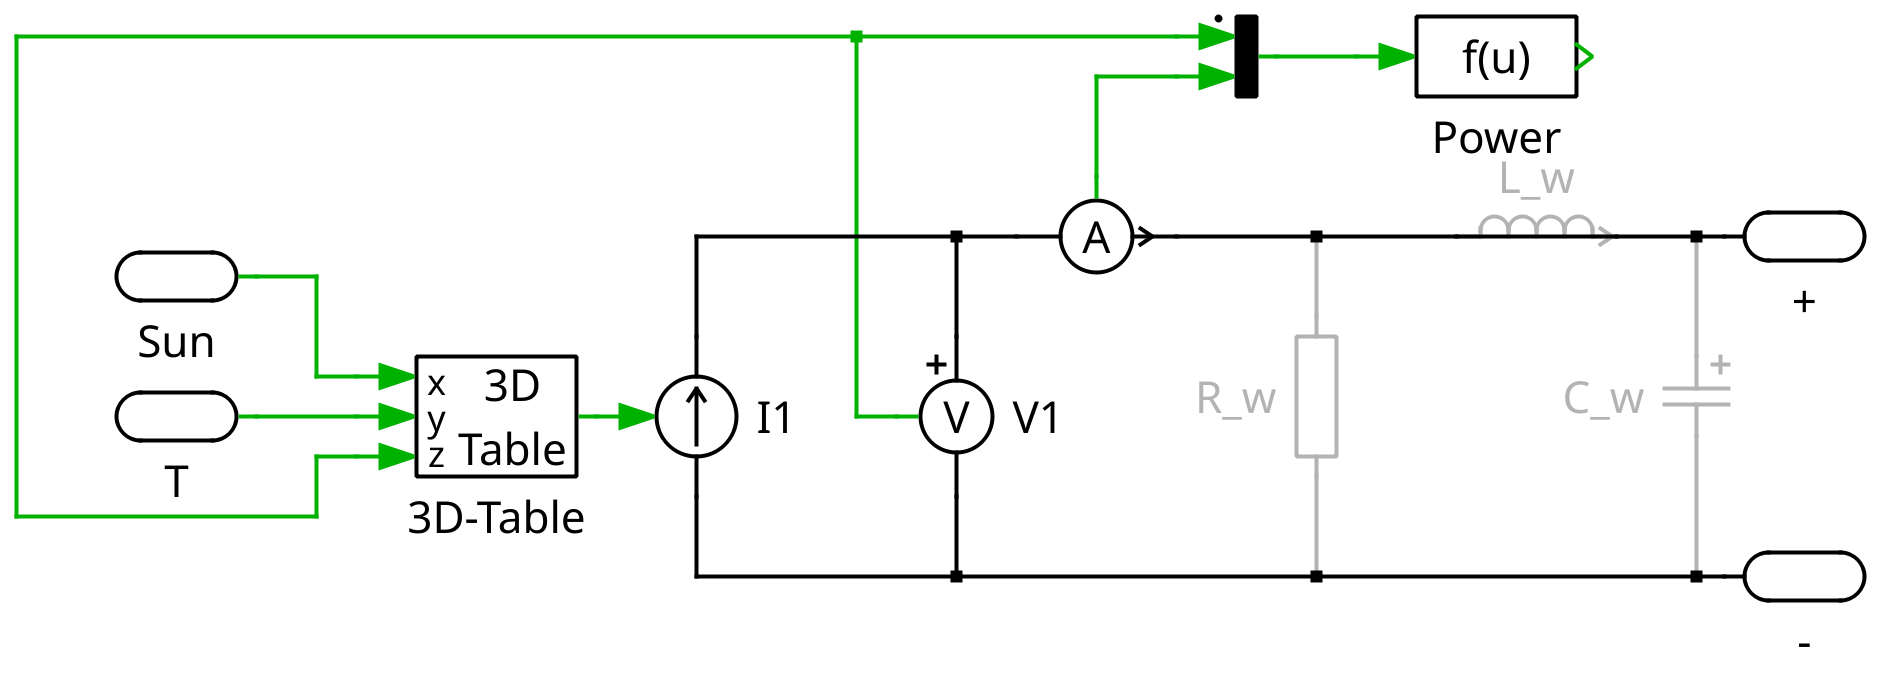
\includegraphics[width=0.7\linewidth]{PV_string}
				\caption{PV Modul als Subsystem in Plecs}
				\label{fig:pvstring}
			\end{figure}
			
		
		\subsection{Einbindung des LUT in Plecs}
			Um ein LUT in Plecs zu verwenden, muss es bei der Initialisierung des PV-Blocks geladen werden. Der Befehl \enquote{load('pv\_lut');} wird dafür im Mask Editor unter dem Reiter \enquote{initialization} eingefügt. Der Mask Editor kann STRG + M aufgerufen werden.\\
			
			Als nächstes werden die Blockparameter des 3D-Table angepasst. Zunächst muss der Array Name angegeben werden. Hierbei ist zu beachten, dass damit nicht der Dateiname des LUTs gemeint ist. Es handelt sich um den Namen des Arrays innerhalb von \enquote{pv\_lut.mat}. Dieser wurde bereits der Arraydeklaration im Octave-Skript Zeile 61 festgelegt.\\
			Bleibt noch die Bestimmung der Vektoren für die x,y,z Parameter. In diesem Fall sind die Daten im LUT folgendermaßen formatiert:\\
			Der Parameter x entspricht der Sonneneinstrahlung, y ist die Temperatur und z die Spannung. Der Vektor muss entsprechend der Menge, sowie Wertebereich eines Parameters angegeben werden:
			\begin{center}
				[Minimum:Schrittweite:Maximum]
			\end{center}
			Beispielhaft für die Sonneneinstrahlung, welche im LUT von 0 bis 1000W/m² hinterlegt ist und insgesamt 10 Stützstellen hat:
			\begin{center}
				[0:100:1000]
			\end{center}
			Damit wird die Ideale Stromquelle entsprechend der Look-up Tabelle gesteuert und alle Schritte zu einer erfolgreichen Simulation eines PV-Moduls durchgeführt.
			
	\newpage
	\printbibliography
\end{document}